\documentclass[11pt]{article}
\usepackage[margin=1in]{geometry}
\usepackage{amsmath,amssymb,graphicx,booktabs,array,hyperref,lineno,float}
\usepackage[T1]{fontenc}
\usepackage{caption}
\usepackage{listings,xcolor}
\lstdefinestyle{wl}{basicstyle=\ttfamily\scriptsize,breaklines=true,breakatwhitespace=false,
  columns=fullflexible,keepspaces=true,showstringspaces=false,frame=single,framerule=0.3pt,rulecolor=\color{black!40},
  numbers=left,numberstyle=\tiny,numbersep=4pt,xleftmargin=1.2em,
  commentstyle=\color{black!55}\itshape,stringstyle=\color{blue!50!black},
  morecomment=[s]{(*}{*)},morestring=[b]",
  postbreak=\mbox{$\hookrightarrow$\space}}
\lstnewenvironment{wlcode}{\lstset{style=wl}}{}
\captionsetup{font=small,labelfont=bf}
\graphicspath{{../figures/}}
\hypersetup{colorlinks=true,linkcolor=black,citecolor=black,urlcolor=blue!50!black}
\linenumbers
\newcommand{\wlTests}{31}
\newcommand{\wlPassed}{31}
\newcommand{\pythonTests}{15}
\newcommand{\pythonLegacyMaxErr}{\ensuremath{1.7\times10^{-5}}}
\newcommand{\pythonLegacyMedErr}{\ensuremath{5.9\times10^{-10}}}
\newcommand{\pythonMaxErr}{\ensuremath{1.2\times10^{-11}}}
\newcommand{\pythonMedErr}{\ensuremath{6.6\times10^{-16}}}
\newcommand{\wlMaxErr}{\ensuremath{2.4\times10^{-11}}}
\newcommand{\wlMedErr}{\ensuremath{1.5\times10^{-15}}}
\newcommand{\campN}{200}
\newcommand{\campOK}{200}
\newcommand{\campMed}{\ensuremath{3.9\times10^{-14}}}
\newcommand{\campPninetyfive}{\ensuremath{2.8\times10^{-12}}}
\newcommand{\campMax}{\ensuremath{3.6\times10^{-9}}}
\newcommand{\campBelow}{100\%}
\newcommand{\campTime}{174~ms}
\newcommand{\demoRep}{family~II, \texttt{cn} branch}
\newcommand{\mmaVersion}{15.0.0 for Microsoft Windows}

\makeatletter\newcommand\inputrows[1]{\@@input #1 }\makeatother
\title{NonlinearOscillatorLab: A Python and Wolfram Language Toolkit for Energy-Based Classification, Accurate Period Computation and Closed-Form Solution of Duffing and Cubic--Quintic Oscillators}
\author{Alvaro H. Salas\\[2pt]\normalsize Department of Mathematics and Statistics\\\normalsize Universidad Nacional de Colombia, Sede Manizales, Colombia\\[2pt]\normalsize Corresponding author: \texttt{ahsalass@unal.edu.co}}
\date{Original Software Publication, SoftwareX --- October 2026}
\begin{document}\sloppy\maketitle
\begin{abstract}
NonlinearOscillatorLab is an MIT-licensed toolkit for the autonomous conservative oscillator $\ddot x+ax+bx^3+cx^5=0$, distributed as two cross-validated implementations: a Python package and a Wolfram Language package for Mathematica. Both determine equilibria and turning points, detect separatrix energies, compute periods on bounded energy components and integrate initial-value problems. Periods are obtained from a factored, singularity-free integrand $1/\sqrt{2Q(x)}$, where $E-V(x)=(x-x_-)(x_+-x)Q(x)$, which gives median relative errors of order $10^{-15}$ and at most $3\times10^{-11}$ up to $10^{-6}$ relative distance from a separatrix, and arbitrary precision in the Wolfram implementation. The Wolfram package also provides the author's closed-form representation $x=Ay/\sqrt{1+\lambda y^2+\mu y^4}$, where $y$ is a Jacobi-elliptic solution of a cubic Duffing equation. Verification combines closed-form elliptic periods, the logarithmic separatrix law $T\simeq k\ln(16/|E-E_s|)$, 32-digit reference trajectories and a seeded randomised campaign. All figures in this paper are generated by the bundled Mathematica scripts.
\end{abstract}
\noindent\textbf{Keywords:} research software; Duffing oscillator; cubic--quintic oscillator; Jacobi elliptic functions; energy methods; period computation; Wolfram Language; reproducibility.

\section*{Code metadata}
\small
\begin{tabular}{@{}p{0.43\textwidth}p{0.5\textwidth}@{}}\toprule
Current code version & v0.1.0\\
Permanent link to code repository & \url{https://github.com/alvarohumberto/NonlinearOscillatorLab}\\
Reproducible capsule & Not available\\
Legal code license & MIT\\
Code versioning system & git\\
Languages, tools, services & Python (NumPy, SciPy, pytest); Wolfram Language (Mathematica / Wolfram Engine)\\
Requirements & Python 3.10+; Mathematica or Wolfram Engine 14.0+ (tested with 15.0 on Windows 64-bit)\\
Developer documentation & README.md; demo notebook in \texttt{mathematica/}\\
Support email & ahsalass@unal.edu.co\\\bottomrule
\end{tabular}
\normalsize

\section{Motivation and significance}
Since Duffing's monograph \cite{duffing}, one-dimensional nonlinear oscillators have remained standard reference systems in mechanics, optics, plasma physics and computational dynamics. Despite the apparent simplicity of the Duffing equation, multiple wells, turning points and separatrices make even the period a quantity that depends on the connected component of the energy surface containing the initial state. Cubic--quintic restoring forces add triple wells and further orbit families. A dependable tool must therefore keep numerical time integration, root identification, energy diagnostics, period evaluation and analytic solution apart, rather than assume that every initial-value problem is periodic or that one formula covers every orbit.

NonlinearOscillatorLab provides these tasks through a small, inspectable API in two languages. The Python package, built on NumPy and SciPy \cite{numpy,scipy}, serves scripted and continuous-integration workflows; the Wolfram Language package adds exact and arbitrary-precision arithmetic, Jacobi-elliptic special functions and the author's closed-form solver for the cubic--quintic equation. Because both implementations expose the same operations, every published number can be computed twice by independent code. This cross-verification revealed a loss of accuracy of the endpoint-substitution quadrature near separatrices (up to \pythonLegacyMaxErr{} relative error in a pre-release version), which motivated the factored integrand now used by both implementations (Section~\ref{sec:period}).

\section{Software description}
\subsection{Model and architecture}
The package treats the initial-value problem
\begin{equation}\ddot x+a x+b x^3+c x^5=0,\qquad x(0)=x_0,\quad \dot x(0)=v_0,\end{equation}
with potential and conserved energy
\begin{equation}V(x)=\frac{a}{2}x^2+\frac{b}{4}x^4+\frac{c}{6}x^6,\qquad E=\frac12\dot x^2+V(x).\end{equation}
Table~\ref{tab:api} lists the corresponding functions; Appendix~\ref{app:wl} gives the Wolfram Language reference, usage examples and complete source code. Equilibria solve $x(a+bx^2+cx^4)=0$ and turning points solve $V(x)=E$, both through polynomial roots in $y=x^2$; inexact roots are polished by Newton steps. In the Wolfram implementation exact coefficients yield exact equilibria (e.g.\ $\{-1,-1/\sqrt3,0,1/\sqrt3,1\}$ for the triple well $a=1,b=-4,c=3$). \texttt{classify\_energy} reports minima, maxima and whether $E$ coincides with a barrier energy; a period is returned only when a unique bounded component $[x_-,x_+]$ containing $x_0$ is identified, and a failure is reported otherwise.

\begin{table}[H]\centering\footnotesize
\caption{Corresponding functions of the two implementations.}\label{tab:api}
\begin{tabular}{@{}lll@{}}\toprule
Task & Python (\texttt{nonlinear\_oscillator\_lab}) & Wolfram Language \\\midrule
Model, $V$, force, $E$ & \texttt{Model(a,b,c)} & \texttt{NOLModel[a,b,c]}, \texttt{NOLPotential}, \texttt{NOLEnergy}\\
Equilibria & \texttt{stationary\_points} & \texttt{NOLStationaryPoints} (exact if possible)\\
Energy classification & \texttt{classify\_energy} & \texttt{NOLClassifyEnergy}\\
Turning points & \texttt{turning\_points} & \texttt{NOLTurningPoints}, \texttt{NOLBoundedComponent}\\
Period & \texttt{period} & \texttt{NOLPeriod} (any \texttt{WorkingPrecision})\\
Closed-form Duffing period & --- & \texttt{NOLDuffingExactPeriod}\\
Closed-form solution & --- & \texttt{NOLExactSolution}, \texttt{NOLDuffingSolution}\\
Time integration & \texttt{simulate} (DOP853) & \texttt{NOLSimulate} (explicit RK, order 8)\\
Energy drift & \texttt{energy\_drift} & \texttt{NOLEnergyDrift}\\
Phase portrait & --- & \texttt{NOLPhasePortrait}\\\bottomrule
\end{tabular}\end{table}

\subsection{Singularity-free period quadrature}\label{sec:period}
For a regular orbit oscillating in $[x_-,x_+]$ the period is $T(E)=2\int_{x_-}^{x_+}dx/\sqrt{2(E-V(x))}$. Since $x_\pm$ are simple roots of the polynomial $E-V$, one may write exactly
\begin{equation}E-V(x)=(x-x_-)(x_+-x)\,Q(x),\qquad Q>0 \text{ on } [x_-,x_+],\end{equation}
where $Q$ is a polynomial of degree at most four obtained by polynomial division. With $x=\bar x+h\sin\theta$, $\bar x=(x_++x_-)/2$, $h=(x_+-x_-)/2$, one has $(x-x_-)(x_+-x)=h^2\cos^2\theta$ and therefore
\begin{equation}T(E)=2\int_{-\pi/2}^{\pi/2}\frac{d\theta}{\sqrt{2\,Q(\bar x+h\sin\theta)}}.\label{eq:Tfactored}\end{equation}
The integrand of (\ref{eq:Tfactored}) is smooth and free of the cancellation $E-V(x)\to0$ that affects the plain substitution at the endpoints. Near a separatrix $Q$ develops a narrow minimum where the orbit passes the barrier; the quadrature is split at the corresponding angles $\theta_k=\arcsin((x_k-\bar x)/h)$ of the stationary points $x_k\in(x_-,x_+)$. In the Wolfram implementation all steps run at a user-selected \texttt{WorkingPrecision} with 20 guard digits.

\subsection{Closed-form references and solutions}
For $c=0$ the package provides the classical elliptic periods
\begin{align}
T&=\frac{4K(m)}{\sqrt{a+bA^2}},\qquad m=\frac{bA^2}{2(a+bA^2)}\qquad (x=A\,\mathrm{cn}(\omega t\,|\,m)),\\
T&=\frac{2K(m)}{A\sqrt{b/2}},\qquad m=2+\frac{2a}{bA^2}\qquad (x=A\,\mathrm{dn}(\omega t\,|\,m),\ \text{intra-well}),
\end{align}
where $A$ is the right turning point and $K$ the complete elliptic integral of the first kind in the parameter convention \cite{byrd,dlmf}. Near the barrier of the double well $a=-1,b=1$ the period obeys $T\simeq k\ln(16/|E-E_s|)$, with $k=1$ for intra-well and $k=2$ for inter-well orbits; both laws are used as independent tests.

For the full cubic--quintic equation, \texttt{NOLExactSolution} implements the author's representation
\begin{equation}x(t)=\frac{A\,y(t)}{\sqrt{1+\lambda y(t)^2+\mu y(t)^4}},\qquad \ddot y+p\,y+q\,y^3=0,\label{eq:cq}\end{equation}
in which the parameters $(A,\lambda,\mu,p,q,\dot y(0))$ follow from the real roots of the cubic $hP^3-aP^2-\tfrac b2P-\tfrac c3=0$, $h=2E$ \cite{salascq}. Two families arise ($\mu=0$ and $\mu\neq0$). The Duffing solution $y$ is selected from the $\mathrm{cn}$, $\mathrm{dn}$, $\mathrm{sech}$ and $\mathrm{sn}/\mathrm{cn}$ branches by \texttt{NOLDuffingSolution}, and a time shift handles initial states at rest at a pole of $y$. Candidates are accepted only after consistency checks on $x(0)$, the local Taylor expansion and the first integral $\dot x^2=2(E-V(x))$; when no real representation passes them a \texttt{Failure} object is returned.

\subsection{Simulation and diagnostics}
Trajectories are integrated with SciPy's \texttt{DOP853} \cite{scipy,hairer} or with Mathematica's \cite{wolfram} eighth-order explicit Runge--Kutta method with dense output of the same order (\texttt{InterpolationOrder->All}). The normalised energy drift is $\delta_E=\max_j|E_j-E_0|/(1+|E_0|)$.

\section{Illustrative examples}
Figure~\ref{fig:pot} shows the five reference potentials used throughout, with their equilibria computed by \texttt{NOLStationaryPoints}; Figure~\ref{fig:phase} shows phase portraits with separatrices obtained from \texttt{NOLClassifyEnergy}. Figure~\ref{fig:closed} compares the closed form (\ref{eq:cq}) with numerical solutions for the demonstration case $a=1,b=0.4,c=0.2$, $x_0=0.8$, $v_0=0.1$ (representation: \demoRep) and for triple- and double-well orbits; panels (b) and (d) give pointwise errors against a 32-digit \texttt{NDSolve} reference. Figure~\ref{fig:pe} shows period--energy curves of all eight orbit families, including the divergence at the separatrices.

\begin{figure}[H]\centering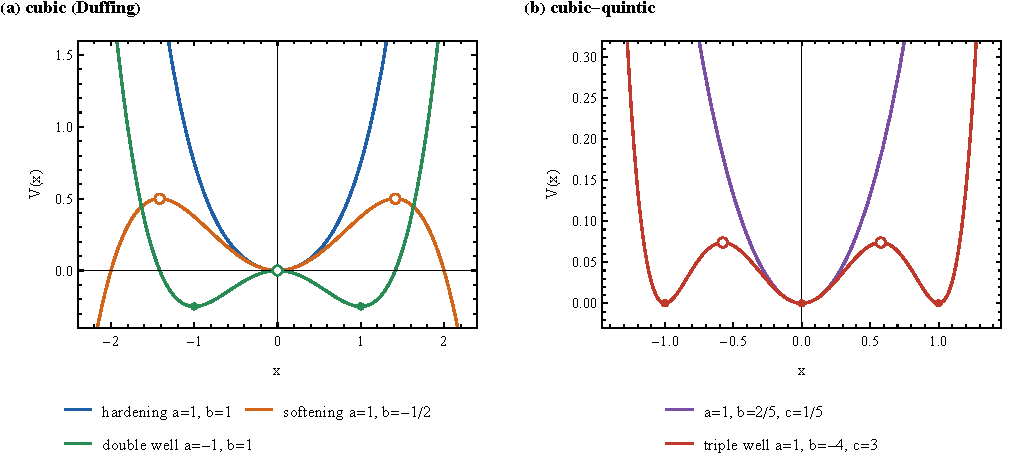
\includegraphics[width=\linewidth]{fig1_potentials.pdf}
\caption{Potentials $V(x)$ for (a) the Duffing cases and (b) the cubic--quintic cases. Filled dots: minima; open circles: maxima (barriers).}\label{fig:pot}\end{figure}

\begin{figure}[H]\centering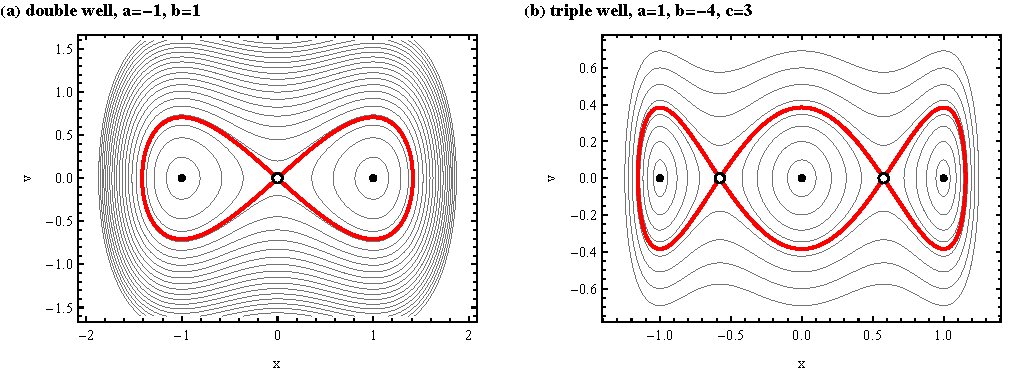
\includegraphics[width=\linewidth]{fig2_phase_portraits.pdf}
\caption{Energy level sets in the phase plane; separatrices (red) pass through the barriers. (a) Double well; (b) triple well with barrier energy $2/27$.}\label{fig:phase}\end{figure}

\begin{figure}[H]\centering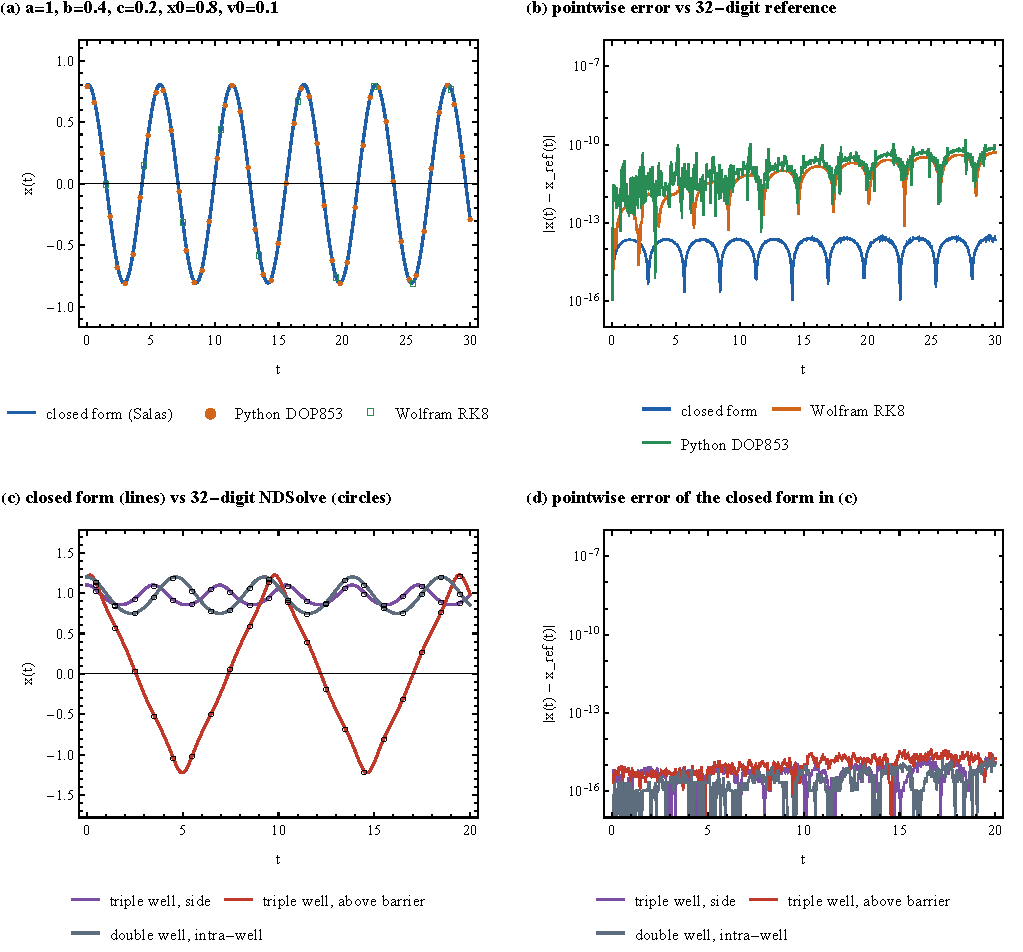
\includegraphics[width=\linewidth]{fig3_closed_form_vs_numerics.pdf}
\caption{(a) Closed-form solution (\ref{eq:cq}) and numerical solutions for $a=1,b=0.4,c=0.2,x_0=0.8,v_0=0.1$. (b) Pointwise deviation from a 32-digit reference for the closed form, the Wolfram RK8 integrator and the Python DOP853 integrator. (c) Closed form versus 32-digit reference for three further orbits and (d) its pointwise error.}\label{fig:closed}\end{figure}

\begin{figure}[H]\centering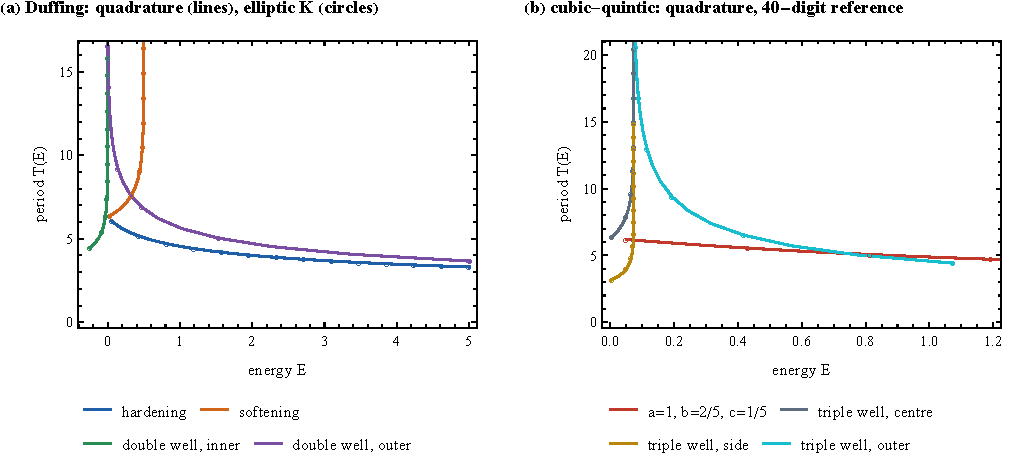
\includegraphics[width=\linewidth]{fig5_period_energy.pdf}
\caption{Period--energy curves. Lines: machine-precision quadrature (\ref{eq:Tfactored}); circles: (a) closed-form elliptic periods, (b) 40-digit quadrature.}\label{fig:pe}\end{figure}

\section{Verification}
\textit{Automated tests.} The Python suite contains \pythonTests{} tests, and the Wolfram suite (\texttt{RunTests.wls}) contains \wlTests{} tests; on \mmaVersion{} \wlPassed{} of \wlTests{} pass, and all Python tests pass. They cover the harmonic reference, exact equilibria, separatrix detection, elliptic periods (machine and 50 digits), the elliptic solutions, the separatrix law, orbit closure $x(T)=x_0$, the closed form (\ref{eq:cq}) on eight orbits, and agreement with the Python periods.

\textit{Period accuracy.} Figure~\ref{fig:acc}(a) shows the relative error of 320 periods (8 families, 40 energies each, approaching the separatrices up to $10^{-6}$ relative distance) against closed-form elliptic values ($c=0$) or 40-digit quadrature ($c\neq0$). The factored integrand gives median errors of \pythonMedErr{} (Python) and \wlMedErr{} (Wolfram), and maximum errors of \pythonMaxErr{} and \wlMaxErr{}, compared with \pythonLegacyMaxErr{} for the endpoint-substitution quadrature. Figure~\ref{fig:acc}(b) confirms the separatrix law down to $|E-E_s|=10^{-16}$. Table~\ref{tab:bench} lists nine benchmark periods to 16 digits.

\textit{Closed-form solver.} Figure~\ref{fig:camp} reports a seeded campaign (\texttt{SeedRandom[20261019]}) of \campN{} random problems with $a,b\in[-12,12]$, $c\in[0,1]$, $x_0\in[-2,0]$, $v_0\in[-2,2]$, the parameter ranges of the author's original test script. A real representation was found in \campOK{} cases (median construction time \campTime{}); on $[0,20]$ the deviation from a 28-digit reference has median \campMed{}, 95th percentile \campPninetyfive{} and maximum \campMax{}, and \campBelow{} of all cases are below $10^{-8}$.

\textit{Precision and tolerance.} Figure~\ref{fig:prec}(a) shows that the number of correct digits of the Wolfram period, measured against an 80-digit value, is at least the requested \texttt{WorkingPrecision}, and Figure~\ref{fig:prec}(b) shows the RK8 energy drift over $[0,200]$ as a function of \texttt{PrecisionGoal}.

\begin{table}[H]\centering\scriptsize\setlength{\tabcolsep}{3.5pt}
\caption{Benchmark periods ($T$, 40-digit Wolfram quadrature, 16 digits shown), relative deviation of the Python and Wolfram machine-precision periods, and maximum deviation of the closed form (\ref{eq:cq}) on $[0,20]$ from a 32-digit reference.}\label{tab:bench}
\begin{tabular}{@{}lrrrrrlccc@{}}\toprule
case & $a$ & $b$ & $c$ & $x_0$ & $v_0$ & $T$ & Python & Wolfram & closed form\\\midrule
\inputrows{../tables/benchmark_periods.tex}
\bottomrule\end{tabular}\end{table}

\begin{figure}[H]\centering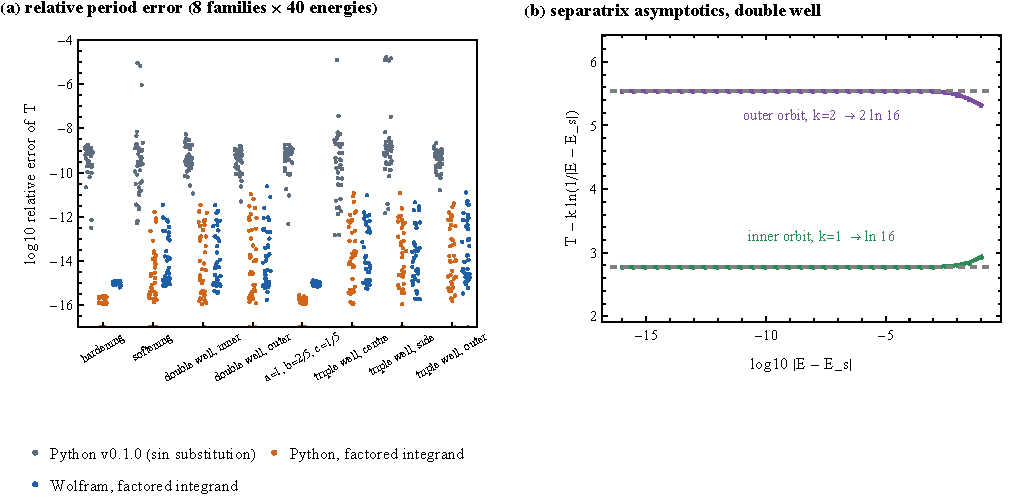
\includegraphics[width=\linewidth]{fig6_period_accuracy.pdf}
\caption{(a) Relative period error for 8 families $\times$ 40 energies: endpoint-substitution quadrature (pre-release Python), factored quadrature in Python and in the Wolfram Language. (b) $T-k\ln(1/|E-E_s|)$ for the double well at 40 digits, converging to $\ln16$ ($k=1$) and $2\ln16$ ($k=2$).}\label{fig:acc}\end{figure}

\begin{figure}[H]\centering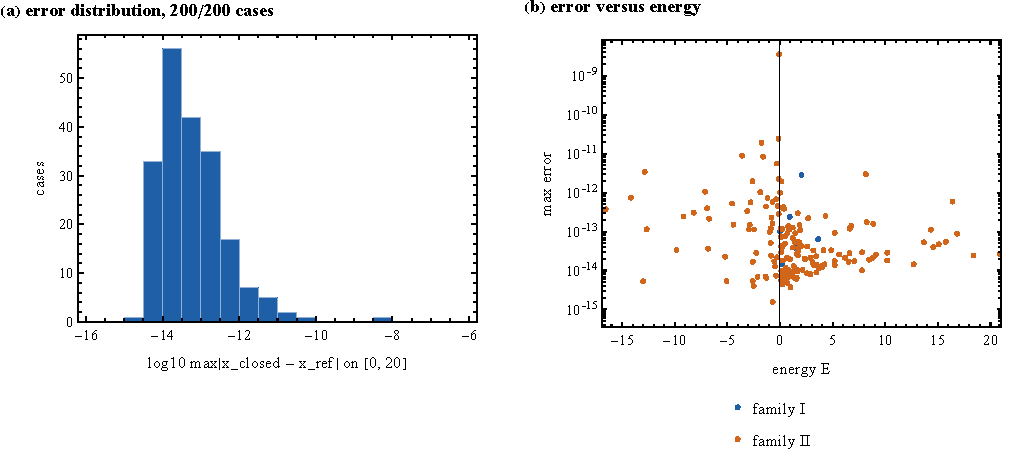
\includegraphics[width=\linewidth]{fig4_closed_form_campaign.pdf}
\caption{Randomised test of the closed-form solver (\ref{eq:cq}): (a) distribution of the maximum deviation from a 28-digit reference on $[0,20]$; (b) deviation versus energy, by representation family.}\label{fig:camp}\end{figure}

\begin{figure}[H]\centering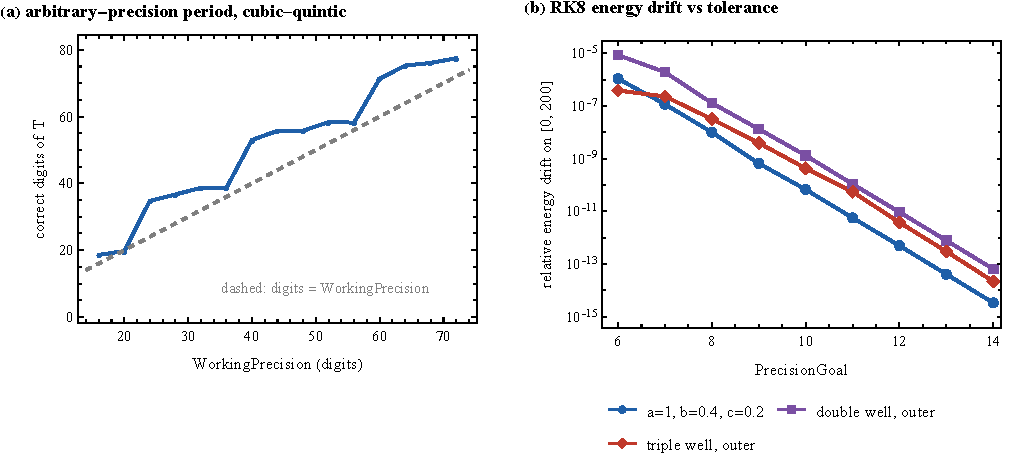
\includegraphics[width=\linewidth]{fig7_precision_and_tolerance.pdf}
\caption{(a) Correct digits of the arbitrary-precision period versus \texttt{WorkingPrecision} for $a=1,b=2/5,c=1/5,x_0=4/5,v_0=1/10$. (b) Energy drift of the RK8 integrator versus \texttt{PrecisionGoal}.}\label{fig:prec}\end{figure}

\section{Impact and reuse potential}
Researchers can use the package as an independent control when developing perturbation series, harmonic-balance, Jacobi-elliptic or other analytic approximations for Duffing-type equations, since it supplies closed forms, machine-precision periods and arbitrary-precision references within one API. The dual implementation lets a computation be repeated in a second language, and the scripts that produce every figure and table of this paper are part of the distribution (\texttt{mathematica/RunAll.wls}, \texttt{benchmarks/}). Teaching applications include phase-plane interpretation, separatrix asymptotics, multi-well potentials and numerical-tolerance studies. No claims of existing adoption or external users are made for this initial release.

\section{Limitations and future work}
The software does not handle damping, forcing, unilateral contact or coupled oscillators, and it provides no interval-certified error bounds. Period evaluation requires simple turning points; exactly at a separatrix the period is reported as infinite and multiple-root cases are rejected. The closed-form solver is currently available only in the Wolfram Language; its coverage is empirical (Figure~\ref{fig:camp}), and for initial states without a real representation it returns a failure rather than an approximation. Planned work includes a Python port of the closed-form solver, event handling and interval enclosures.

\section*{Availability and reproducibility}
The Python package, the Wolfram Language package, test suites, benchmark scripts and the figure-generating scripts accompany this manuscript as an MIT-licensed archive. Running \texttt{wolframscript -file mathematica/RunAll.wls} regenerates every figure and table. Appendix~\ref{app:wl} documents the Wolfram Language package, its usage, and lists its complete source code. The source code is publicly available at \url{https://github.com/alvarohumberto/NonlinearOscillatorLab}.
\section*{CRediT authorship contribution statement}
Alvaro H. Salas: Conceptualization, Methodology, Software, Validation, Writing -- original draft, Writing -- review and editing.
\section*{Declaration of competing interests}
The author declares no known competing financial interests or personal relationships that could have appeared to influence the work.
\section*{Funding}
No external funding is declared.
\section*{Data availability}
No external research datasets were used. All data shown are generated by the scripts included with the code archive.
\clearpage
\begin{thebibliography}{9}
\bibitem{duffing} G. Duffing, \emph{Erzwungene Schwingungen bei ver\"anderlicher Eigenfrequenz und ihre technische Bedeutung}, Vieweg, Braunschweig, 1918.
\bibitem{salascq} A. H. Salas, \textbf{[ADD: reference for the closed-form cubic--quintic representation $x=Ay/\sqrt{1+\lambda y^2+\mu y^4}$]}.
\bibitem{byrd} P. F. Byrd, M. D. Friedman, \emph{Handbook of Elliptic Integrals for Engineers and Scientists}, 2nd ed., Springer, Berlin, 1971.
\bibitem{dlmf} NIST Digital Library of Mathematical Functions, Chapter 22: Jacobian Elliptic Functions, \url{https://dlmf.nist.gov/22}.
\bibitem{scipy} P. Virtanen et al., SciPy 1.0: Fundamental algorithms for scientific computing in Python, \emph{Nature Methods} 17 (2020) 261--272. \url{https://doi.org/10.1038/s41592-019-0686-2}.
\bibitem{numpy} C. R. Harris et al., Array programming with NumPy, \emph{Nature} 585 (2020) 357--362. \url{https://doi.org/10.1038/s41586-020-2649-2}.
\bibitem{hairer} E. Hairer, S. P. N{\o}rsett, G. Wanner, \emph{Solving Ordinary Differential Equations I: Nonstiff Problems}, 2nd ed., Springer, Berlin, 1993.
\bibitem{wolfram} Wolfram Research, Inc., Mathematica, Version 15.0, Champaign, IL, 2026.
\end{thebibliography}

\clearpage
\appendix
\nolinenumbers
\section{Wolfram Language (Mathematica) implementation and usage}\label{app:wl}
This appendix documents the Wolfram Language package \texttt{NonlinearOscillatorLab.wl} and the scripts that produce every figure and table of the paper. The code was run with Mathematica~15.0 on Windows 64-bit, and Mathematica or Wolfram Engine 14.0 or later is required. The complete source is listed in Sections~\ref{app:src}--\ref{app:figs}; the same files are in the \texttt{mathematica/} folder of the software archive.

\subsection{Installation and running}
No installation is needed. Download or clone the repository (\url{https://github.com/alvarohumberto/NonlinearOscillatorLab}), or copy the folder \texttt{mathematica/} anywhere, and load the package by file name:
\begin{wlcode}
Get["C:/path/to/NonlinearOscillatorLab/mathematica/NonlinearOscillatorLab.wl"]
NOLVersion        (* "0.1.0" *)
\end{wlcode}
The verification suite, the figures and the tables are reproduced from a terminal with \texttt{wolframscript},
\begin{wlcode}
wolframscript -file mathematica/RunTests.wls      (* 31 tests -> test_report.txt / .csv *)
wolframscript -file mathematica/MakeFigures.wls   (* figures/*.pdf, *.png; tables/*.csv, *.tex *)
wolframscript -file mathematica/RunAll.wls        (* both *)
\end{wlcode}
or from a notebook with \texttt{Get["\dots/mathematica/RunAll.wls"]}. \texttt{MakeFigures.wls} reads the Python reference data in \texttt{benchmarks/} and \texttt{examples/orbit.csv}, so Python is not needed to rebuild the figures. A full run takes about 3--4 minutes on a laptop; most of the time is spent in the 200 reference integrations of the randomised campaign. \texttt{MakeDemoNotebook.wls} writes the tutorial notebook \texttt{NonlinearOscillatorLab\_Demo.nb}.

\subsection{Function reference}
Table~\ref{tab:wlref} summarises the public functions. A model is the inert expression \texttt{NOLModel[a,b,c]} (\texttt{NOLModel[a,b]} sets $c=0$). Exact coefficients and initial data (integers, rationals, radicals) give exact equilibria and turning points and allow any \texttt{WorkingPrecision}; machine numbers give machine-precision results. Functions that cannot return a meaningful value return a \texttt{Failure} object and issue a message, so results can be tested with \texttt{FailureQ}.

\begin{table}[H]\centering\footnotesize
\caption{Public functions of \texttt{NonlinearOscillatorLab.wl}.}\label{tab:wlref}
\begin{tabular}{@{}p{0.39\textwidth}p{0.57\textwidth}@{}}\toprule
Call & Result\\\midrule
\texttt{NOLPotential[m,x]}, \texttt{NOLForce[m,x]}, \texttt{NOLEnergy[m,x,v]}, \texttt{NOLCurvature[m,x]} & $V(x)$, $-V'(x)$, $\tfrac12v^2+V(x)$, $V''(x)$\\
\texttt{NOLStationaryPoints[m]} & sorted real roots of $V'(x)=0$\\
\texttt{NOLClassifyEnergy[m,x0,v0]} & Association with keys \texttt{"Energy"}, \texttt{"Equilibria"}, \texttt{"Minima"}, \texttt{"Maxima"}, \texttt{"OnSeparatrixEnergy"}\\
\texttt{NOLTurningPoints[m,E]} & sorted real roots of $V(x)=E$\\
\texttt{NOLBoundedComponent[m,x0,v0]} & $\{x_-,x_+\}$ enclosing $x_0$, or \texttt{Failure}\\
\texttt{NOLPeriod[m,x0,v0]} & period by Eq.~(\ref{eq:Tfactored}); \texttt{Infinity} at equilibria; \texttt{Failure} on separatrices or unbounded motion. Options: \texttt{WorkingPrecision}, \texttt{PrecisionGoal}, \texttt{"Tolerance"} (default $10^{-9}$)\\
\texttt{NOLPeriodFromEnergy[m,E,x0]} & period of the energy-$E$ orbit through the well containing $x_0$\\
\texttt{NOLDuffingExactPeriod[a,b,A]} & closed-form $K(m)$ period for $c=0$ and turning point $A$\\
\texttt{NOLDuffingExactSolution[a,b,A,t]} & $A\,\mathrm{cn}$ or $A\,\mathrm{dn}$ solution with $x(0)=A$, $\dot x(0)=0$\\
\texttt{NOLSeparatrixPeriodAsymptotics} \texttt{[m,xs,dE,k]} & leading term $(k/\lambda)\ln(1/|dE|)$, $\lambda=\sqrt{-V''(x_s)}$\\
\texttt{NOLDuffingSolution[p,q,y0,y1]} & closed-form solution of $\ddot y+py+qy^3=0$ (case label, modulus, frequency, period or blow-up time, \texttt{"y"})\\
\texttt{NOLExactSolution[m,x0,v0]} & closed form (\ref{eq:cq}); key \texttt{"x"} is a pure function of $t$, plus representation data, or \texttt{Failure}\\
\texttt{NOLExactSolutionError} \texttt{[m,x0,v0,sol,tmax]} & $\max|x_{\rm closed}-x_{\rm ref}|$ on $[0,t_{\max}]$ against a 32-digit \texttt{NDSolve} reference\\
\texttt{NOLSimulate[m,x0,v0,tEnd]} & \texttt{<|"x","v","tEnd",\dots|>} from an 8th-order explicit Runge--Kutta method with dense output; options \texttt{WorkingPrecision}, \texttt{PrecisionGoal}, \texttt{AccuracyGoal}, \texttt{Method}\\
\texttt{NOLEnergyDrift[m,sol]} & $\delta_E=\max_j|E_j-E_0|/(1+|E_0|)$ on 2001 samples (option \texttt{"Samples"})\\
\texttt{NOLPhasePortrait[m,\{x1,x2\},\{v1,v2\}]} & energy level sets with separatrices in red; option \texttt{"Levels"} and all \texttt{ContourPlot} options\\\bottomrule
\end{tabular}\end{table}

\subsection{Usage examples}
The outputs shown in comments are those obtained with Mathematica~15.0; the period values agree with Table~\ref{tab:bench}.

\subsubsection*{Energy geometry.}
\begin{wlcode}
m = NOLModel[1, -4, 3];                 (* triple well *)
NOLStationaryPoints[m]                  (* {-1, -1/Sqrt[3], 0, 1/Sqrt[3], 1}   exact *)
NOLPotential[m, 1/Sqrt[3]]              (* 2/27   barrier energy *)
NOLClassifyEnergy[m, 1/2, 0]["Maxima"]  (* {{-1/Sqrt[3], 2/27}, {1/Sqrt[3], 2/27}} *)
NOLBoundedComponent[m, 1.1, 0.]         (* {x-, x+} of the side-well orbit *)
NOLPhasePortrait[m, {-1.35, 1.35}, {-0.75, 0.75}, "Levels" -> {0.01, 0.04, 0.07, 0.1, 0.15}]
\end{wlcode}

\subsubsection*{Periods at machine and arbitrary precision.}
\begin{wlcode}
NOLPeriod[NOLModel[1, 0.4, 0.2], 0.8, 0.1]                       (* 5.633261676532774 *)
NOLPeriod[NOLModel[1, 2/5, 1/5], 4/5, 1/10, WorkingPrecision -> 50]  (* 50-digit value *)
{NOLPeriod[NOLModel[-1, 1], 1.2, 0], NOLDuffingExactPeriod[-1, 1, 1.2]}
                                    (* {4.623905221811913, 4.623905221811913} *)
NOLPeriod[NOLModel[-1, 1], 1, 2^(-1/2)]   (* message NOLPeriod::sep, returns Failure *)
NOLPeriod[NOLModel[1, -1], 2., 0]         (* message NOLPeriod::unb, returns Failure *)
\end{wlcode}
Exact input is required for high precision: with \texttt{NOLModel[1,0.4,0.2]} the result would only carry machine precision, because $0.4$ is a machine number; use \texttt{NOLModel[1,2/5,1/5]} instead.

\subsubsection*{Closed-form solution of the cubic--quintic equation.}
\begin{wlcode}
m   = NOLModel[1, 0.4, 0.2];
sol = NOLExactSolution[m, 0.8, 0.1];
sol["Representation"]           (* "II / y: cn: orbit around 0" *)
KeyDrop[sol, {"x", "y"}]        (* A, lambda, mu, Duffing p and q, y(0), y'(0), ... *)
sol["x"][3.]                    (* x(3) from x = A y/Sqrt[1 + lambda y^2 + mu y^4] *)
NOLExactSolutionError[m, 0.8, 0.1, sol, 20]   (* about 3*10^-14 on [0, 20] *)
Plot[sol["x"][t], {t, 0, 30}, Exclusions -> None]
\end{wlcode}
\texttt{Exclusions -> None} is recommended when plotting the closed form, because the representation contains \texttt{Abs} and \texttt{Sign}, which \texttt{Plot} would otherwise treat as possible discontinuities.

\subsubsection*{Simulation and energy drift.}
\begin{wlcode}
s = NOLSimulate[NOLModel[-1, 1], 1.6, 0, 100];
NOLEnergyDrift[NOLModel[-1, 1], s]                   (* relative drift on [0, 100] *)
s = NOLSimulate[NOLModel[-1, 1], 1.6, 0, 100, PrecisionGoal -> 14, AccuracyGoal -> 16];
Plot[{s["x"][t], s["v"][t]}, {t, 0, 100}]
\end{wlcode}

\subsubsection*{Separatrix asymptotics.}
\begin{wlcode}
m = NOLModel[-1, 1]; dE = 10^-12;
NOLPeriodFromEnergy[m, -dE, 1, WorkingPrecision -> 40, "Tolerance" -> 10^-30] -
  NOLSeparatrixPeriodAsymptotics[m, 0, dE, 1]        (* -> Log[16] = 2.7725887... *)
\end{wlcode}
A smaller \texttt{"Tolerance"} is needed here because the default $10^{-9}$ would classify an energy $10^{-12}$ below the barrier as lying on the separatrix.

\subsection{Package source: \texttt{NonlinearOscillatorLab.wl}}\label{app:src}
The closed-form solver (\texttt{duffingSolution}, \texttt{cqCandidates}, \texttt{cqBuild}, \texttt{cqSolution}) is the author's original code, kept verbatim inside the package.
\lstinputlisting[style=wl]{../mathematica/NonlinearOscillatorLab.wl}

\subsection{Verification suite: \texttt{RunTests.wls}}\label{app:tests}
\lstinputlisting[style=wl]{../mathematica/RunTests.wls}

\subsection{Figures and tables: \texttt{MakeFigures.wls} and \texttt{RunAll.wls}}\label{app:figs}
\lstinputlisting[style=wl]{../mathematica/MakeFigures.wls}
\lstinputlisting[style=wl]{../mathematica/RunAll.wls}

\end{document}
